% Source file:
% https://kwarc.eecs.iu-bremen.de/repos/jacobs/research-report/ses/input/belov_alexei/Alexei Belov-2.doc

\subsubsection{Interlocking structures, Algebra}
\label{is:belov}
\index{Belov, Alexei}

\paragraph{Research Team}
Alexei Belov (Visiting Professor)

\medskip

My research deals with the following fields of mathematics:
\begin{enumerate}
\item {\sl Interlocking structures.}
  For any two-dimensional arrangement of convex figures there is one which can
  be shifted away without touching the others.  However, in 3D-space this is
  not always possible: there exist interlocking structures. They can be used in
  mechanics. Crack propagation stops on the boundary of grains, and on the
  other hand, grains can support each other. This effect provides new
  possibilities in constructing new materials.

\item {\sl Polynomial authomorphisms and quantization.}
  The famous Jacobian conjecture has important relations with quantization. The
  quantization approach, relations between the Weyl algebra and Poisson
  brackets, is very promising.

\item {\sl Polynomial identities and finite basis problem.}
  The Specht problem asks whether a given set of identities is already a
  consequence of a finite subset.
\end{enumerate}

\paragraph{Highlights} {\sl Interlocking structures.} Consider a set of
contacting convex figures in ${\mathbb R}^2$. It is not difficult to prove that
one of these figures can be moved out of the set by translation without
disturbing the others. Therefore, any set of planar figures can be disassembled
by moving the figures \emph{one by one}. One may think that this statement
holds for higher dimensions as well. However, attempts to generalize it to
${\mathbb R}^3$ have been unsuccessful. As a counterexample, structures
consisting of convex solid bodies which cannot be disassembled by removing
individual bodies were suggested by G.A.~Gal'perin in~1985.

Rather unexpectedly, interlocking assemblies of all types of regular
polyhedra were discovered recently. See Figures \ref{fig:belov-fig2}
and~\ref{fig:belov-fig6}.

%Consider an infinite layer of cubes. The middle section of the layer produces a
%square lattice. Let us color the section in a checkerboard fashion. Now, we
%alter the inclinations of lateral faces of the cubes pairwise. Consider for
%instance a `black' cube, i.e.\ a cube associated with a black cell of the
%lattice. Incline the `north' and `south' faces of the cube outwards at an
%angle~$\alpha$, together with the faces of the two adjacent cubes. With a
%proper choice of the angle~$\alpha$, a cube is transformed to a tetrahedron and
%the entire layer turns into an  assembly of interlocked tetrahedra,
%Fig.~\ref{fig:belov-fig2}.

%\begin{figure}[ht]
%\begin{center}
%  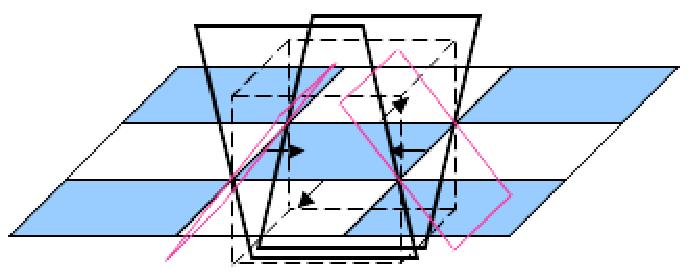
\includegraphics[width=7cm]{Belov/belov-fig1}
%\end{center}
%\mycaption{Modification of cube faces. The arrows show the sense of the
%           inclinations of
%  the modified faces.}\label{fig:belov-fig1}
%\end{figure}

\begin{figure}[ht]
\begin{center}
  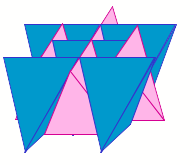
\includegraphics[width=7cm]{Belov/belov-fig2}
\end{center}
\mycaption{Fragment of interlocking set of tetrahedra.}\label{fig:belov-fig2}
\end{figure}

\begin{figure}[ht]
\begin{center}
  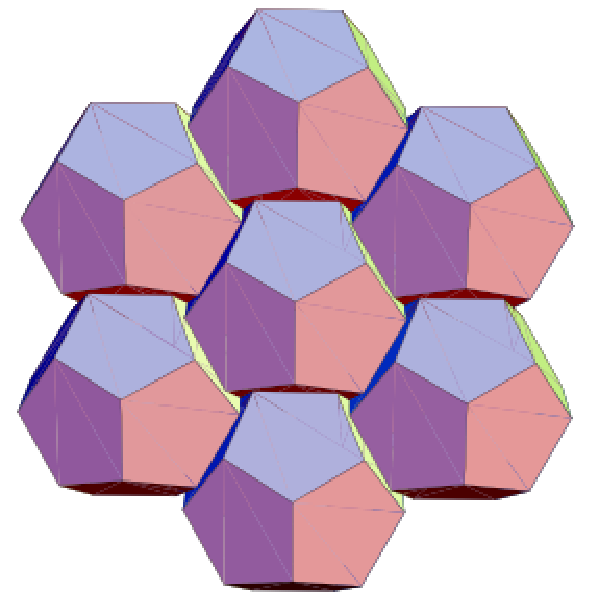
\includegraphics[width=7cm]{Belov/belov-fig6}
\end{center}
\mycaption{Fragment of interlocking set of dodecahedra normal to the symmetry
           axis of 3rd order.}\label{fig:belov-fig6}
\end{figure}

%The appropriate inclinations of the faces of the constituent elements are the
%key feature of interlocking structures.

The above structure provides an example of an assembly in which no element can
be removed without disturbing its neighbors. It is appealing to use such
arrangements in engineering as a new design principle. This principle allows
one to build structures of convex elements without a binder phase or
connectors, i.e., structures that (a)~possess high resistance to fracture
propagation (fractures getting stopped at interfaces between the elements) and
(b)~are free of stress concentrations associated with mechanical connectors
used in conventional assemblies of building blocks (Fig.~\ref{fig:belov-fig6}).
%Thus, there is a practical need to find and characterize interlocking sets. The
%structures described are obtained by tiling the plane with equal squares.
%A.J.
%Kanel-Belov considered another regular tiling -- the hexagonal (honeycomb) one
%and found a new type of interlocking solids, which turn out to be simple
%cubes!
A.J.~Kanel-Belov found a new type of interlocking structures built
from simple cubes. It is surprising that such a structure, which could
have been known since antiquity, was only discovered recently.
% It might be known in ancient time, but not!



%\begin{figure}[ht]
%\begin{center}
%  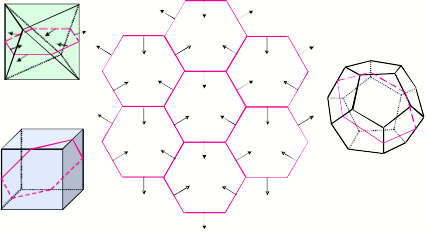
\includegraphics[width=7cm]{Belov/belov-fig3}
%\end{center}
%\mycaption{Hexagonal tiling of the plane and the associated platonic solids
%           with their respective hexagonal middle sections. Orientations of
%           arrows indicate the inclinations of faces of the modified hexagonal
%           prisms that provide their interlocking.}\label{fig:belov-fig3}
%\end{figure}

%\begin{figure}[ht]
%\begin{center}
%  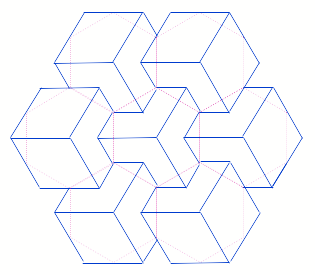
\includegraphics[width=7cm]{Belov/belov-fig4}
%\end{center}
%\mycaption{Fragment of interlocking set of cubes.}\label{fig:belov-fig4}
%\end{figure}

%\begin{figure}[ht]
%\begin{center}
%  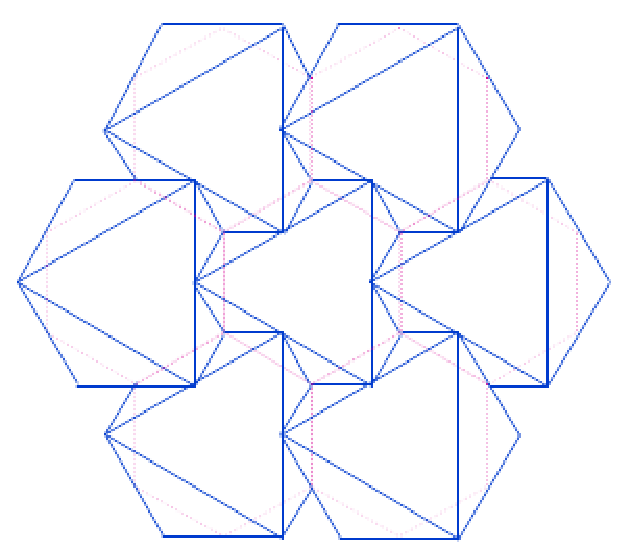
\includegraphics[width=7cm]{Belov/belov-fig5}
%\end{center}
%\mycaption{Fragment of interlocking set of octahedra.}\label{fig:belov-fig5}
%\end{figure}

%\begin{figure}[ht]
%\begin{center}
%  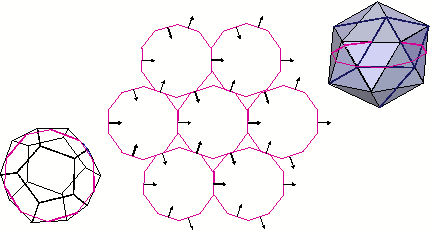
\includegraphics[width=7cm]{Belov/belov-fig7}
%\end{center}
%\mycaption{Decagonal tiling of plane and the associated dodecahedron and
%           icosahedron. Only arrows that correspond to contacting faces are
%           shown.}\label{fig:belov-fig7}
%\end{figure}

The diversity of interlocking arrangements of regular convex polyhedron
uncovered so far suggests that there might be a whole wealth of such structures
beyond the examples presented. These structures
%, as well as conventional
%masonry structures, cracked solids, blocky rock masses and some asteroids and
%comets are all examples of fragmented bodies. Considerations presented show a
%way to develop a geometric theory of fragmented bodies. Such a theory
could
also shed light on some interesting natural phenomena, e.g., the integrity and
mechanics of flexible sandstones or ancient building techniques, like dry stone
walling and may have some exciting engineering applications, such as a new
concept of protective tiles for the Space Shuttle.

\smallskip

{\sl Jacobian Conjecture and quantization.}

Let $F: {\mathbb C}^n\to {\mathbb C}^n$ be a polynomial mapping. If it is
invertible, then the Jacobian determinant of~$F$ is a non-zero constant.
According to the {\sl Jacobian Conjecture $(JC_n)$} from~1934, this condition
should be sufficient.

Let $W_n$ be the Weyl algebra of polynomial differential operators in $n$
variables over~${\mathbb C}$. The {\sl Dixmier conjecture $(DC_n)$} from~1967
says that {\it every endomorphism of $W_n$ is an authomorphism}.

Recently A.J.~Belov and M.L.~Kontsevich proved that these two
conjectures are equivalent
(another proof was independently obtained by Y.~Tsuschimoto).
The idea of proof is based on reduction to positive characteristic and
consideration of Poisson brackets on the center of Weil algebra
modulo~$p$.
This new approach to studying polynomial authomorphisms is based on
quantization.
%Let $A$ be an associative commutative algebra endowed with Poisson brackets.
%The Kontsevich quantization theorem says that there exists a
%deformation $*$ of the multiplication in~$A[[h]]$ such that $x*y$ is equivalent
%to $xy \mbox{mod} h$, and $(x*y-y*x)/h$ is equivalent to $\{x,y\}$.
%
%The Weyl algebra $W_n$ is a quantum space. It is the result of quantization of
%the polynomial ring via the standard Poisson bracket.  The Kontsevich
%conjecture states that the group of polynomial authomorphisms of ${\mathbb
%C}^n$ is isomorphic to the group of authomorphisms of the Weyl algebra.
%% It means equivariant properties of quantization.
%
%In the proof that the Jacobian and Dixmier Conjectures are equivalent, a
%homomorphism between these two groups was constructed. It is important to
%notice that we use deformation in an arithmetic direction (where a prime number
%plays role of the Planck constant).

\smallskip

{\sl Polynomial identities and Specht problem.}
A {\sl polynomial identity} of an algebra~$A$ is a polynomial which vanishes on
this algebra. An identity~$g$ is a consequence of a set of identities ${f_i}$
if any algebra that satisfy the system ${f_i}$ also satisfies~$g$.

Many classes of algebras can be axiomatized as a class of algebras satisfying
some identities. The {\sl Specht problem} asks whether every set of identities
is a consequence of a finite subset.

In characteristic~0 the answer is~{\sl Yes}, as was shown by A.~Kemer. In
general, the answer is~{\sl No}, it was shown by A.~Belov. But if the number of
generators is bounded, then the answer is~{\sl Yes}, as was shown by A.~Belov.
The last result was recently accepted by `Izvestia of Russian Academy of Science.'

\paragraph{Organization}

\begin{enumerate}
\item Training weekend for the German IMO team at Jacobs University Bremen
      (with D.~Schleicher and M.~Stoll)
\end{enumerate}

\paragraph{Collaborations}
\begin{enumerate}
\item {\sl Institut des Hautes Etudes Scientifiques, Bures sur Yvette, France}\\
  Prof.~M.L.~Kontsevich \\
  Polynomial authomorphism theory
\item {\sl Hong-Kong University} \\
  Prof.~Yu Jietai \\
  Polynomial authomorphism theory
\item {\sl Wayne State University Detroit, USA} \\
  Prof.~L.~Makar-Limanov \\
  Polynomial authomorphism theory
\item {\sl University of California, San Diego, USA} \\
  Prof.~E.~Zelmanov \\
  Polynomial authomorphism theory
\item {\sl Bar-Ilan University, Israel} \\
  Prof.~L.~Rowen and Prof.~U.~Visshnu\\
  Polynomial Identities and Specht problem
\item {\sl Moscow State University, Russia} \\
  Prof.~V.N.~Latyshev and Prof.~A.V.~Michalev \\
  Polynomial Identities and Specht problem \\
  Ph.~Dr.~I.~Ivanov \\
  Interlocking structures
\item {\sl University of Western Australia} \\
  Prof.~A.V.~ Dyskin and Dr.~E.~Pasternak \\
  Interlocking structures
\item {\sl  Technische Universit\"at Clausthal, Germany} \\
  Prof.~J.~Estrin, \\
  Interlocking structures
\end{enumerate}

\paragraph{Grants}
\begin{enumerate}
\item Funded by Israel Science foundation, \emph{ Grant
``Polynomial Identities''}
      No.~1178/06.
\end{enumerate}

%\paragraph{Publications}
% Source file:
% https://kwarc.eecs.iu-bremen.de/repos/jacobs/research-report/ses/input/belov_alexei/publications-belov.tex
\nocite{Belov5}
%\nocite{Belov6}
\nocite{Belov7}
%\nocite{Belov8}
%\nocite{Belov9}
%\nocite{Belov10}

%\end{document}
%%% Local Variables:
%%% mode: latex
%%% TeX-master: "report"
%%% End:
